\section{Field Study}
\label{sec:field-study}


	The field study took place during the first two weeks of March, from 3/3/2015 to 3/15/2015 in a faculty building of Ludwig-Maximilians-University Munich. Data was collected on 14 consecutive days and personal semi-structured interviews were carried out on five working days during the same two weeks. A total of 117 interactions were registered with the application installed on the public display and 58 survey responses were recorded.

	The goal of this study was to validate the previous thoughts, get better insights into our research questions, and to see how users respond to questionnaires being conducted on displays in the public.




\subsection{Research Questions}

	% MOTIVATE: explain why we make this field study, explain what we hope to expect. what are our assumptions. what did we expect from the questionnaires, what did we expect from the interviews?

	One of the main reasons why we performed this field study was to get a better understanding of our assumptions and hypotheses. Especially since there is often a discrepancy between what one assumes and what can actually be observed in real world. This phenomena has already been stated in the publication by Ojala and Kostakos in 2011: ``Introduction A common criticism targeted at many studies on interactive public displays is that their evaluation usually takes place in non-realistic lab environments, and for short periods of time. Thus, a long-term real- world deployment could be a more appropriate evaluation.''\cite{Ojala2011}.

	% Why did we bother to do this study?
		% to find out if our results and predictions validate in the field

	% What do we assume
	% What do we want to know
		% which variables are there, how do we expect them to change?

	The assumption we made for the development of our first research prototype of the PDSurvey platform is that we can simplify the conduction and deployment of surveys to large public display networks. Since this is a rather large claim, we broke down the hypothesis to multiple more fine-grained statements. The claim, whether the PDSurvey platform facilitates the conduction of large-scale surveys in public, will be evaluated in the following chapter (see chapter \ref{sec:expert-interview}). 

	What we will evaluate in the scope of this thesis, are the following research questions:

	\begin{enumerate}
	\item Which question types are best suited for questionnaires carried out in public? How should a survey be constructed to take best advantage of the PDSurvey platform? (quantitative vs. qualitative)

	\item Which channels are most suited for completing surveys (on a digital platform) in public?
		% The first step was to ask ourselves the question, which channel is suited for gathering responses from the audience. ...

		% We already had an application running on a public display in a faculty building which attracted lots of regular and new users. Our interest was how we could best integrate questionnaires on and after the application itself (a balloon shooter game).
	\item (assessed between the lines) What motivated our users to fill in surveys?
	\end{enumerate}


	Research questions which would go beyond the scope of this thesis, and might serve as follow-up questions for further research are gathered here:

	\begin{itemize}
	\item In which situations is the user most willing to answer surveys on public displays?
	\item (not really copious): how many questions are acceptable, the attention span would be of great interest
	\item (not really copious): how the users noticed / perceived the survey
	\item (Not treated): where to position the survey on screen. As stated in a paper by J\"org M\"uller ... TODO reference it TODO ..., the best position on large public displays is directly in the center (not at the bottom, not at the top, close to the center). The larger the screen is, the more relevant a centric positioning will get.
	\item (Not treated): The influence of the environment on which question types are suited, how personal the questions can get, how much privacy the display should offer (the smaller the display, the more private the context seems)
	\item (Not treated): How can we best break down a standardized survey with 10+ questions and spread a subset of the questions across multiple users?
	\end{itemize}

	In addition to these questions we were also interested in user stories, in the feedback real-world users gave us in regards to answering surveys on screens in the public. For this reason we also conducted semi-structured interviews in parallel to the quantitative evaluation of the PDSurvey platform.




\subsection{Study Setup}
	% = METHOD Section
	% give the reader enough information to replicate the experiment
	% consists of 1 Design, 2 Participants, 3 Apparatus, 4 Procedure

	Both quantitative and qualitative data was gathered as part of the field study. Quantitative data was obtained through the PDSurvey system and qualitative data was collected through semi-structured interviews. To facilitate comparison between quantitative and qualitative data some quantitative questions were asked redundantly at the end of the semi-structured interview.

	\subsubsection{Design}

	Our primary goal was to find out which channel the users preferred, the questions they had to answer in the questionnaire played a secondary role. The survey displayed on all four channels contained the same five questions. 

	\begin{itemize}
	\item How often have you used this display before? [number]
	\item How likely is it that you will use this display in the future again? [5-point Likert scale]
	\item Which devices do you possess or use regularly? [multiple choice with 5 check boxes]
	\item In which area do you study / work? [text field]
	\item What was your motivation for approaching and using this display? [text field]
	\end{itemize}

	In order to also get first insights into how well certain question types are suited for surveys in public, where a short completion time is crucial, we varied between the following question types and kept them in the same order: numerical question, Likert scale (single click), multiple choice (based on check boxes) and two text fields for an undefinied length of the response. To increase the motivation for participation we stated that the questionnaire consists of five questions, will only take one minute to complete and is for the Master's thesis of student at LMU Munich (see figure \ref{fig:5-pdclient-intro}).
	As proven by Richard Ryan in his self-determination theory\cite{ryan2000self}\footnote{http://www.selfdeterminationtheory.org/}, this additional intrinsic motivation increased the participation and acceptance rate of the public survey additionally. 

	\begin{figure}
	    \begin{center}
	        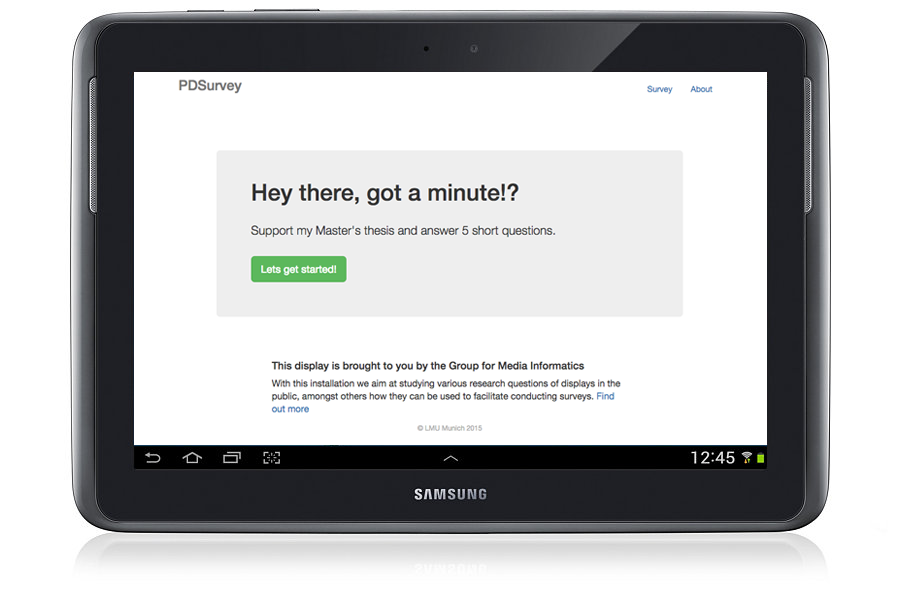
\includegraphics[width=.7\columnwidth]{img/5_field-study/pdclient-startscreen.png}
	    \end{center}
	 \caption{PDClient: Motivating users to participate in a short questionnaire}
	 \label{fig:5-pdclient-intro}
	\end{figure}

	To find out more about the motive we carried out semi-structured interviews on location.



	THIS PART outlines the formal structure of the study. identifies the experiments dependent and independent variables.
	also state here which study design I have chosen: 1 independent-measures, repeated-measures, mixed-design

		\begin{enumerate}
		\item provide an overview of the overall structure of your experiment. 
		\item what were the independent variables in the study? what were the factors that I manipulated? >> none! 
		\item how many conditions were there: ... i would say none, since I didn't vary any parameters
		\item describe what was measured, what were the dependent variables?
		\item >>> I would actually say, that I didn't carry out any experiment, I only made an observation with evaluation. I didn't vary any parameters, I only configured a study setup and observed + interviewed the participants
		\end{enumerate}




	\subsubsection{Participants}
		% provide the necessary information about the people who took part in your experiment

		In total 54 questionnaires were completed and 28 semi-structured interviews were conducted during the two week study period.

		\textit{Questionnaires} were completed by a random number of people with different backgrounds. What they all had in common was their affiliation to LMU Munich, either because of being a student, staff or otherwise related (parents, pensioner, industry partner). Since our research focus was on finding which feedback channel is best suited for conducting automated questionnaires in public, we only included one question to collect demographic data. Based on the fourth question (In which area do you study / work?) it can be seen, that most of the participants are doing something related to computer science.
			+++ describe the rest of the data, refer to a table +++
		 ... 
			54 submissions, 43 non-empty submissions which could be assigned to a study field.

		For the participants in the \textit{semi-structured interview} demographic data was also collected. Out of the 28 participants
		20 were male and 18 were female. The age of all people interviewed ranged between 20 and 69, with an average age of 31,5 years.
		Due to the wide variety of faculties and the public library located in the building, various technical backgrounds were present. Two retirees, three workers and 23 students were interviewed. The study fields which were most frequently represented are computer science (4), japanology (4), ethnology (3), political science (3). Besides that students studying sociology, communication science, law, physics or engineering were interviewed.


		\begin{table}[h]
		\begin{tabular}{lllll}
		   & \textbf{people participated in survey} &  &   & \textbf{people interviewed}             \\
		10 & Informatics                            &  & 4 & Informatics                             \\
		6  & Political Science                      &  & 4 & Japanology                              \\
		5  & Anthropology                           &  & 3 & Ethnology                               \\
		4  & Cultural Science                       &  & 3 & Political Science                       \\
		4  & Business                               &  & 1 & Communication Science                   \\
		2  & Physics                                &  & 1 & Sociology                               \\
		2  & Sociology                              &  & 1 & Law                                     \\
		1  & Ethnology                              &  & 1 & Physics                                 \\
		1  & Communication Science                  &  & 1 & Engineering                             \\
		1  & Sports                                 &  & 3 & workers (PhD, public officer, SysAdmin) \\
		1  & Science and Technology                 &  & 2 & in pension          
		\end{tabular}

		\begin{tablenotes}
      		\small
      		 \item Sample description underneath the table. 
		\end{tablenotes}
		\caption[Demographics of Field Study]{Demography for the survey data (left) and the semi-structured interview (right).}
		\label{table:demographics}
		\end{table}


		\begin{enumerate}
		\item give details on how many participants you used
		\item how many took part in which condition
		\item include information about demographic values (age, gender)
		\item also deliver brief details on how you obtained the participants: they didn't get any reward for participating. XX were passerby, XX participated in the game from their own motivation.
		\item describe the population of my participants. what was their background?
		\item  Before starting the interviews the people participating and passing by were asked whether they noticed the option to fill in a survey, and XX out of XX didn't notice the option. 
		\item think about which information is relevant. for me the devices they possess might be of relevance. people not possessing a smartphone or tablet, might be less willing to use these devices.  
		\end{enumerate}


		% + differentiate between 
		% 1) on its own completed questionnaire
		% 2) semi-structured interview

		In regards to the semi-structured interview the participants can be differentiated into three groups: participants who approached the display by themselves (and were observed doing so), people passing by the display (noticing the display, however not approaching it) and the last group of people simply passing by (not having noticed the display). To increase the amount of feedback, we approached people from all three groups. The distribution between the group was as follows: 9 direct participants, 17 passerby (XX observed, XX didn't approach it)
		The number of surveys was not explicitly increased thereby.




	\subsubsection{Apparatus}
		% give details of any equipment used, including thinkgs like questionnaires and other tests

		The apparatus consisted of a XXX-inch TV screen, a Samsung Galaxy tablet, two questionnaires (one for participants, one for passerby), a voice-recorder (smartphone), and the client of the PDSurvey platform installed on the TV screen and on the tablet. The TV screen and the tablet to the right of it (see figure \ref{fig:5-study-setup}) were there permanently, the other devices only while conducting semi-structured interviews.


		\begin{figure}
		    \begin{center}
   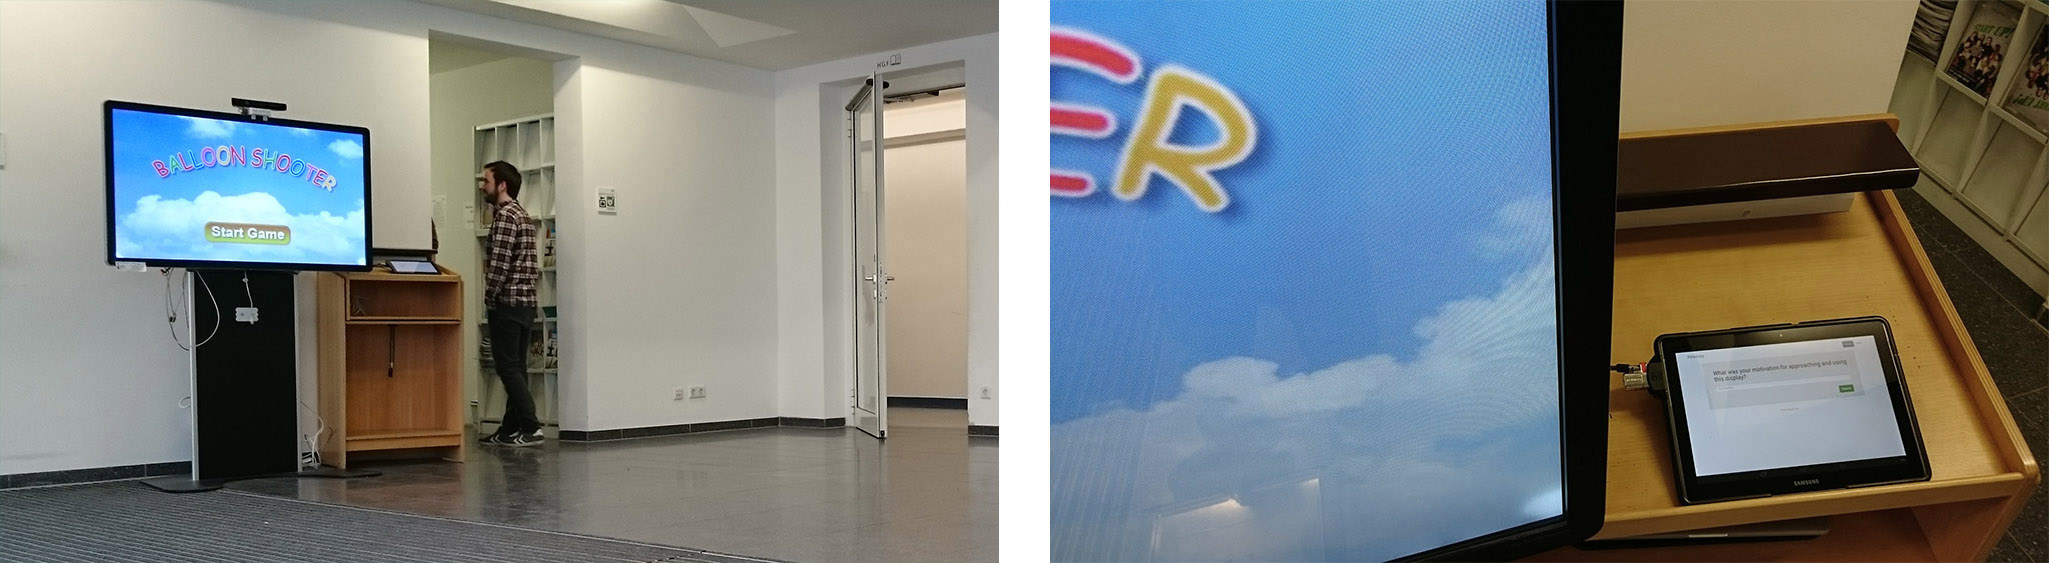
\includegraphics[width=\columnwidth]{img/5_field-study/study-setup.jpg}
		    \end{center}
		 \caption{Overview of the study setup in the entrance hall of the faculty building.}
		 \label{fig:5-study-setup}
		\end{figure}

		Our object of investigation was the TV screen with touch support, running an interactive \textit{Balloon Shooter} game. After users completed the game, they were asked via a notice inside of the game to fill in a questionnaire on one of the four provided feedback channels. 
		

		Each user had the opportunity to respond directly on the TV display (1), on a tablet to the right of the big TV (2), via their own smartphone (3) or via email (4). The first option was embedded directly into the Balloon Shooter game, offering a consistent UI and the most direct feedback channel. Choosing the tablet as an option, the users were prompted to move to the right and to answer five questions on the tablet. The Samsung Galaxy Tab 10.1 was displaying the responsive frontend of PDClient, being enclosed in a Android Kiosk App, namely KioWare Lite\footnote{http://www.kioware.com/android.aspx}. Choosing the option to use a smartphone prompted the user to either scan a QR code or to access a URL. The last option consisted of an input field embedded into the Balloon Shooter game on the TV screen, asking the user to enter their email address. The address was logged from inside of the game to a txt-file which was scanned every 5 minutes by a Windows task scheduler. For sending the email via SMTP a Python script was used\footnote{https://github.com/lukasziegler/python-send-mail}.Screenshots of all four options can be found in the Appendix on page \pageref{appendix:screenshots-balloon-shooter}.

		For this quantitative part of the evaluation the following data was logged for all four options: The timestamp of the users choice, which feedback channel the user chose to respond to the survey and whether they skipped the call to participate in the survey or if they stopped playing the game (measured via timeout). 
		% For option 1 being chosen (responding directly on the TV screen) all five responses were logged. For options 2 and 3 the user accessed the PDClient frontend, leading to a logging of the data in the RESTful backend. And for option 4, responding via email, the email address was logged In the case that options 2 to 4 were chosen, all data was directly collected on the PDSurvey platform itself.


		% maybe also show a flow of actions, but not sure if this is needed, when the user can also simply read the previous paragraph.


		For the evaluation in the field study itself a self-made questionnaire was used, since the focus was on finding which channels and question types are best suited in general for being used on public display. This was the reason why we did not use any of the standardized questionnaires mentioned in section \ref{sec:questionnaires}. The questionnaires used can be found in the Appendix.


		% + give more information about the balloon shooter game.
		% + ask Jiamin, whether and which screenshots of the game I am allowed to post?

		More information regarding the Balloon Shooter game can be found here XXXXX. 
		The main application installed on the public display was a game called \textit{Balloon Shooter} developed and run by Jiamin Shi, a PhD student at the Group for Media Informatics at LMU Munich. It was first installed on January 7th 2015 and has been running in different versions since then. Public audience was already used to it for roughly two months and adapted to it well.





	\subsubsection{Procedure}
		% tell the reader how the study was carried out in practice
		= Is this section equivalent to the method section?

		MY FIRST NOTES FOR WRITING

		% Duration
		The field study consisted of a two week gathering of log data. During this time we recorded ...


		% Adjustments on the day prior to the evaluation
		The day prior to the launch of the actual field study was used for assembly and for last adjustments, like change of font size, adjustment to the position of certain UI elements, and for getting indirect feedback from users observing but not approaching the display.
		From observing it could be seen that a more effective call-to-action was needed. Many people looked at the display, noticed that something has changed with the setup, but no one started interacting with the new setup or was willing to complete the questionnaire. Therefore a more catchy start screen was introduced for the tablet (see \ref{fig:5-pdclient-intro}) and the option panel of the TV screen was also modified () see screenshot \ref{screenshot:options}. 
		This observation is very much in line with the findings of Richard Ryan and Edward Deci published as the self-determination theory\cite{ryan2000self}.


		% Instructions


		\begin{enumerate}
		\item How I introduced the scenario to the passerby. Imagine you are in a shopping mall or at an airport using one of those large displays to find some information. In the end you get asked to answer a short questionnaire. (How would you react to it? And to the more qualified students with the right background I also asked how they would feel when getting asked quantitative or qualitative data. / KW-student) 
		\end{enumerate}

		META-INFORMATION FOR THIS CHAPTER
		\begin{enumerate}
		\item This section gives details of how you carried out the experiment in practice.
		\item Describe how you executed your experiment. How you approached the scenario, what you did, which parameters were measured and which conditions/parameters were changed? 
		\item how long were the interviews? 2:30 to 4 minutes
		\item which instructions were given to the participants? none! 
		\item + state how we motivated the users to participate: only 5 questions, results are for a MA thesis

		\end{enumerate}




		% DONT FORGET - only give RELEVANT INFORMATION to the reader!!
		% > only provide details if they are needed for replication
		% > or if they are relevant to the outcome of the experiment




\subsection{Not sure where it belongs to}

	\subsubsection{Location}

	All parts of the field study were carried out in the faculty building for computer science, a building where other research institutes for ethnology, political science, Japanese studies, and physics are also located.

	The study was carried out in the entrance hall of the university building. Figure \ref{fig:5-entrance-hall} shows an excerpt of the universities floor plan for the entrance hall, allowing for a better understanding of the dynamics.

	\begin{figure}
	    \begin{center}
	     \fbox{		        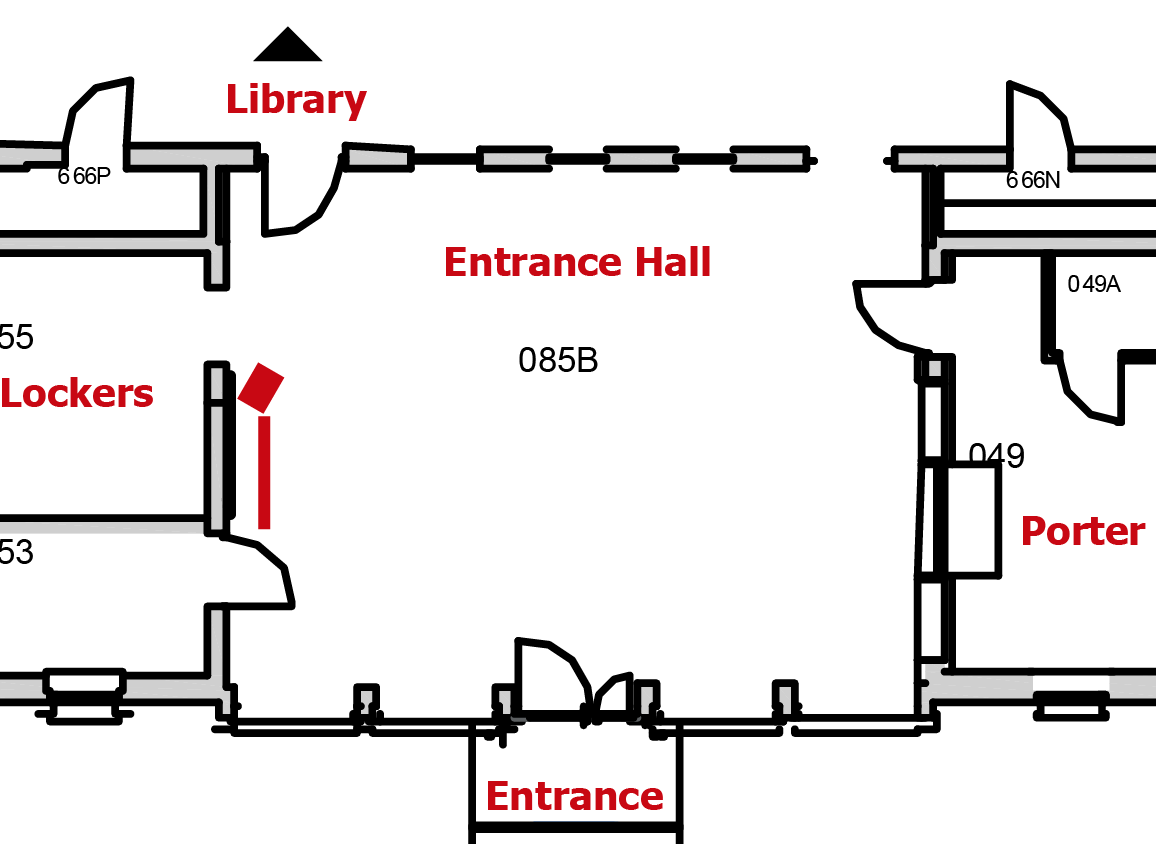
\includegraphics[width=.7\columnwidth]{img/5_field-study/entrance-hall.png}
	     }
	    \end{center}
	 \caption{Floor map of the entrance hall where the field study was carried out. User paths, and the surrounding environment including facilities such as the library can be seen here.}
	 \label{fig:5-entrance-hall}
	\end{figure}

	- which path users choose
	- that they are usually in a hurry
	- having a break
	- or waiting for somebody
	- facilities near by are: the library, smoking area outside, toilets, lockers



	\subsubsection{Limitations}

	\begin{enumerate}
	\item the tablet was always on, it was possible to approach the tablet directly without having the option to participate in the survey via smartphone or email. 
	\item the novelty effect played a role for the first part of the evaluation. It was striking to see a response rate of 50 percent. If we exclude all participants who directly accessed the tablet and skipped the appeal to use one of the four options, there was still a response rate of 10 percent.
	\item all questions were optional, since we wanted to see if people are less willing to respond to certain question types.
	\item incomplete surveys were also allowed and considered for evaluation. It allowed us to get first insights to whether certain questions or question types are more suited than others.
	\end{enumerate}

	Further limitations found on public display installations, stated by Ojala et al. \cite{Ojala2011}, are: location of display, effect of curiosity, impact of novelty, and influence of weather (for outdoor usage). The effect of curiosity and novelty certainly played a role for our field study. Therefore the participation rate in general (and the participations directly on the tablet) were thus higher. For our two primary research questions, which question type and which feedback channels are best suited, the impact of novelty and curiosity should not have a big impact.


	\subsubsection{Conditions}

	No conditions were present, since not a real lab experiment with different conditions was conducted, but a study observing how the user responded to one setting, having four options to fill in a survey:

		\begin{enumerate}
		\item on public display
		\item on tablet, next to the large TV display
		\item via smartphone: 
		\item via email, from home:
		\end{enumerate}


	\subsubsection{Methodology}
		% tell the reader how the study was carried out in practice






\subsection{Results}


\subsubsection{Quantitative Results}
	% Quantitative = pure facts
	% read pages 293, 294 + 327 - 333

	% important, don't interpret any data in this section
	% just tell the reader what you found


% SURVEY DATA

	We received a total of 57 filled in surveys, submitted via all four provided feedback channels. The majority of the surveys were submitted directly on the tablet (87.72\%). 

	% NumQuestions
	% Due to the phenomena described by Alt et al. \cite{TODOTODOTODO}, a minimum number of possible questions needed to be used. We chose to limit the number of questions asked via all four channels to 5, to avoid a low participation and response rate. 

	% Demographics
	Regarding the demographics of the participants only the occupation of each participant can be derived from the questionnaire. As far as was indicated, all people playing with the game in our scenario were students. Majority of people interacting with the TV screen study informatics (23.8\%), followed by political science (14.3\%), japanology (11.9\%), anthropology (11.9\%), cultural science (9.5\%), and business (9.5\%). Table \ref{table:demographics} shows a full list of which study field or work field the participants specified.

	% Likeliness to play / participate again
	The likeliness to use the tablet again for further 

		> for the large TV screen a much smaller number survey responses were recorded, the overall likeliness for using the display again was much higher (average=4.5, median=5, SD=0.87).

	% How often have the users used this display before?

	% Which devices the users possess

	On average 2.4 devices were 

	The following combinations were most frequent:
		12	smartphone, tablet, laptop
		12	smartphone, laptop
		6 	smartphone, laptop, desktop
		3 	only smartphone

	When looking at an aggregated version, allowing the clustering of subsets in between patterns, than the laptop (PERCENTAGE) is the most popular device:
		34 	smartphone + laptop (possibly combined with other devices)
		18	smartphone + tablet
		15	tablet + laptop
		12	smartphone + desktop
		10 	laptop + desktop

	Overall, the majority of the people participating in the survey already owned a smartphone (79.3\%)

		42	smartphone (79.3\%)
		10	feature phone (18.9\%)
		22	tablet (41.5\%)
		39	laptop (73.6\%)
		13	desktop (26.4\%)


%% OBSERVATIONS

Two behaviors noticed during the field study, which match with the insights form Peltonen et al. \cite{peltonen2008s}. On the one hand the interaction with high parallel usage. People tend to share the display space with their friends, they were all interacting with the game at once. Once the game was over and the options for responding to the survey showed up, the more dominant person standing in the middle in front of the screen responded to the questionnaire. Another effect visible was that people using the display attracts more users to participate.
In our scenario most people approached the public display installation directly, skipping the stepwise approach.


%% INTERVIEW DATA

A total of 28 semi-structured interviews were conducted, of which 72.4\% of the participants were male and 28.6\% were female. The average age was 31.5 years, with an age distribution ranging from 20 years up to 69 years (median=25.5, SD=13.2). Eleven of the 28 interviews were conducted with actual participants of the public display study setup (39.3\%), the remaining 17 interviews (60.7\%) consisted of people passing by the display. 

To avoid any interferences between the two groups, each passerby was asked before starting the interview whether he has noticed the public display installation, and whether he has already interacted with the installation. Out of all passerby no one has previously been interacting with the game or survey platform. 82.4\% (14 of 17) of the passerby have already noticed the public display installation before, however, none of the passerby has previously participated in the game. The remaining 17.6\% have neither approached the display nor noticed it previous to the interview. 

Looking at the scientific background of all 28 participants, 79.2\% are students, the remaining 20.8\% either already worked full-time or were in pension. The majority of students studied informatics (16.7\%), japanology (16.7\%), ethnology (12.5\%) or political science (12.5\%).

From what has been mentioned, the main reason for approaching the public displays was in 6 out of 8 cases ``curiosity'' (6x). Two other reasons were ``for fun'' (1x) and ``waiting for someone'' (1x). Reasons for not approaching the display were ``no time'' (2x) and ``it is in the entry zone of the university, it feels strange when one plays with it'' (1x).

% b Channel preferred
Based on the interview data, the 
The most interesting feedback channel for 
B 


FROM DATA
30.77%
46.15%
15.38%
7.69%

FROM INTERVIEW
32.14\%
42.86\%
7.14\%
17.86\%

% c plus reason why





\begin{table}[h]
\center
\begin{tabular}{lllll}
\multicolumn{2}{l}{\textbf{From Survey Data}} &  & \multicolumn{2}{l}{\textbf{From Interviews}} \\
30.77\%                   & \multicolumn{3}{l}{on public display}    & 32.14\%                  \\
46.86\%                   & \multicolumn{3}{l}{on tablet}            & 42.86\%                  \\
15.38\%                   & \multicolumn{3}{l}{on smartphone}        & 7.14\%                   \\
7.69\%                    & \multicolumn{3}{l}{at home / via email}  & 17.86                   
\end{tabular}
\caption[Feedback Channel]{Preferred feedback channel for answering surveys.}
\end{table}



% RANDOM, not sure where to put it

	Pretreatments
	\begin{enumerate}
	\item crossing out any unwanted / distorting data (e.g. the person in pension, who didn't participate, but only argued)
	\item making changes to the data
	\end{enumerate}


	% I) Descriptive Statistics
	% - provide summaries of group performance
	% - present: average, mean, mode
	% - describes: standard deviation, range (how it is spread)
	% - describes: frequency of data (if relevant)

	% presentation of data
	% - don't present data multiple times
	% - either use a TABLE or a GRAPH

	give the reader a clear idea of what you found!


	\begin{enumerate}
	\item For a good SAMPLE of how to list the basic population (x male, y female) of the survey, have a look at paper number 25 from the Appendix. (WIP)
	\item describe the results from the evaluation
	\item e.g. 1) prefered feedback channel, 2) number of acceptable answers, 3) preferred setting
	\item say which implications this gives for the PDSurvey research platform
	\end{enumerate}
	


	% How many questions were completed, which ones were left empty
	The first question (numeric) was completed in all surveys. 

	% ggf. unterscheiden nach den drei Gruppen:
		% 1 participants who approached the display
		% 2 people passing by the display
		% 3 passing by, not having any intention to approach the display


	% >>> look at paper 29: great read, how they deconstructed their interviews and paraphrased all relevant data in a very compact way! <<<

	% >>> reason, that people prefer using smaller displays for more sensitive data, since they feel safer there, has also already been stated by: paper 23 \cite{Huang2004}

	% >>> paper #101 [CHI12BaillyShoeSense.pdf] "ShoeSense" contains another good evaluation



	% II) Inferential Statistics

	% are the results of statistical tests, showing the SIGNIFICANCE between groups and conditions



\subsubsection{Qualitative Results}
	% Qualitative = a combination of facts + evaluation

	ASK WHETHER I SHOULD COMBINE THESE TWO SECTIONS

	%% Evaluation based on Grounded Theory
	% for systematic evaluation of qualitative data (interview transcripts)
	% while having the goal of generating a theory
	% > datengestützte Theoriebildung = auf Empirie bezogene Bildung von Hypothesen / Theorien


	% ggf. unterscheiden nach den drei Gruppen:
		% 1 participants who approached the display
		% 2 people passing by the display
		% 3 passing by, not having any intention to approach the display




\subsection{Discussion}

	% 1) Start with a few sentences that summarize the most important results (+ see \url{http://www.ldeo.columbia.edu/~martins/sen_sem/thesis_org.html}).
	% read pages 295 -  297 + 336 - 341

	\begin{enumerate}
	\item (summarize the expert interviews)
	\item summarize the quantitative results
	\item summarize the qualitative results 
	\item TODO: think about what my evaluation has to do with my platform. make sure that this link is clear! Make this link clear in the following summary.
	\end{enumerate}

	% 2) Now allowing room for interpretation and personal opinions:

	Some of these observations were also in compliance with the five adaptation factors stated by Huang et al. \cite{Huang2004}: task specificity and deep integration, tool flexibility and generality, visibility and exposure to others' interaction, low barriers to use, dedicated core group of users.

	\begin{enumerate}
	\item \textbf{questions in the public} / questionnaires on public displays are best suited for quantitative surveys. Users want a short interaction time, not having to think much about their answers and for roughly XXXXX percent of the participants it holds true, that they do not like being observed while making responses in public.

	\item From this observation, the implication for the \textbf{question types} can be derived: question types ideally with a single-click interaction are preferred (e.g. Likert scale, multiple choice with all options given, yes/no-questions). Then followed by numeric, dropdown and multiple choice questions with an open end. For these question types the user has to think a little bit more, he has to assess more precisely in order to make his response. One example stated by a participant, in regards to the numeric question `How often have you used this display before?', was that ``It would be great if you had the possibility to choose from a predefined range, because typing is not always optimal. I would prefer if areas would be given instead of oneself having to think about the exact number.'' Last, being no big surprise, are text fields combined with open-ended questions. As a take away for text fields: wherever possible rephrase the question so that you can respond to it as short as possible.

	\item and in regards to the \textbf{feedback channel}, no clear recommendation can be made. All offered feedback channels were present in the evaluation and during the semi-structured interviews for each channel a good reason was given. What can be said that the crowd usually distinguishes into three groups. The first (and slightly larger) group preferring the option of \textit{direct response}. They are not as considerate about answering questions in public and their privacy aspect. For them it is more important to complete the survey as quick as possible and not having to think about it later, as long as nothing too private or personal gets asked. One person said ``If something too private would be asked, I would simply abort and go away from the display''. The second group is more privacy concerned, often older of age, or actually wanting to take the time to think about all of their responses in depth in order to give high-quality responses. This group prefers to take the questionnaire away from the public setting into their home. The last group choose the feedback channel purely based on their \textit{habit} and what they are accustomed to. Two ladies in their mid-twenties responded immediately ``on my smartphone, because I am most used to it''.

	\item and regarding the \textbf{display size}: the smaller the display, the safer and more private they feel. An exception to this finding could be old people. Once people become short-sighted or more insecure and unconfident with using new devices, they prefer having a large input surface.

	\end{enumerate}


	Further notes, not sure where to integrate them:
	\begin{enumerate}
	\item ``No amount of upfront analysis would ever have been enough to pre- determine all of the requirements and properties that would be needed. A priori analysis is useful, but only in a systems development environment that also allows for significant changes to happen after actual first pilot testing results have been collected and analyzed.'' \cite{russell2004use}
	\end{enumerate}


	% 3) Restate and make sure, what my evaluation has to do with my platform. make sure that this link is clear!



